%!TEX root = ./template-skripsi.tex
%-------------------------------------------------------------------------------
%                            BAB II
%               TINJAUAN PUSTAKA DAN DASAR TEORI
%-------------------------------------------------------------------------------

\chapter{KAJIAN PUSTAKA}
  
\section{Pengertian Citra Digital}
    Citra digital adalah citra analog yang diubah ke dalam bentuk digital melewati proses, akuisisi,  pengambilan sampel \textit{(sampling)}, dan kuantisasi. Proses akuisisi yaitu proses pemetaan suatu fenomena fisik menjadi citra kontinu dengan menggunakan sensor. Keluaran dari proses akuisisi adalah sebuah gelombang tegangan bersifat kontinu yang amplitudo dan perilaku spasialnya berkaitan dengan fenomena fisik yang ditangkap oleh sensor tersebut. Untuk mendigitalisasi citra tersebut, perlu didefinisikan sebuah fungsi yang mengambil koordinat dan amplitudo sebagai parameternya. Proses \textit{sampling} dan kuantisasi diperlukan untuk mengubah data kontinu tersebut ke dalam bentuk digital. Proses \textit{sampling} adalah proses mendigitalisasi nilai koordinat, sementara kuantisasi adalah proses mendigitalisasi nilai amplitudonya \citep{Gonzalez2018}.
    
    Citra digital tersusun dari banyak \textit{picture element} atau biasa disebut piksel, yang masing-masing bernilai diskrit. Nilai diskrit tersebut merepresentasikan intensitas atau tingkat keabuan \textit{(grayscale)} dari masing-masing piksel. Citra digital dapat didefinisikan sebagai fungsi dua dimensi $f(x, y)$, dimana $x$ dan $y$ melambangkan koordinat spasial dan amplitudo $f$ sebagai nilai intensitas atau tingkat keabuan citra pada koordinat tersebut \citep{Gonzalez2018}.
    
    \begin{equation}\label{eq:2.1}
        f(x, y) = 
        \begin{bmatrix}
        f(0, 0) & f(0, 1) & \cdots & f(0, N - 1)\\
        f(1, 0) & f(1, 1) & \cdots & f(1, N - 1)\\
        \vdots & \vdots & \ddots & \vdots \\
        f(M - 1, 0) & f(M - 1, 1) & ... & f(M - 1, N -1)
        \end{bmatrix}
    \end{equation}
    
    Persamaan \ref{eq:2.1} merepresentasikan citra digital $f(x, y)$ dalam bentuk \textit{array} numerik berukuran $M \times N$, dimana $M$ adalah jumlah baris dan $N$ adalah jumlah kolom. Variabel $x$ dan $y$ pada $(x, y)$ adalah koordinat diskrit yang ditulis menggunakan bilangan integer: $x = 0, 1, 2, \ldots, M - 1$ dan $y = 0, 1, 2, \ldots, N - 1$. Setiap elemen dalam \textit{array} di atas dapat disebut sebagai \textit{image element}, \textit{picture element}, \textit{pel}, atau \textit{pixel}. Citra juga dapat direpresentasikan dalam bentuk matriks tradisional. Bentuk representasi ini adalah yang digunakan untuk memproses citra pada komputer \citep{Gonzalez2018}.
    
    \begin{equation}\label{eq:2.1}
        A = 
        \begin{bmatrix}
        a_{0, 0} & a_{0, 1} & \cdots & a_{0, N - 1}\\
        a_{1, 0} & a_{1, 1} & \cdots & a_{1, N - 1}\\
        \vdots & \vdots & \ddots & \vdots \\
        a_{M - 1, 0} & a_{M - 1, 1} & \cdots & a_{M - 1, N - 1}
        \end{bmatrix}
    \end{equation}
  
\section{Pengolahan Citra Digital}
    Pengolahan citra digital mengacu pada proses manipulasi citra digital menggunakan komputer. Proses ini mengambil citra digital sebagai masukan \textit{(input)} dan menghasilkan keluaran \textit{(output)} berupa citra yang sudah diolah atau dimanipulasi. Dalam bukunya, \citet{Gonzalez2018} membagi pengolahan citra ke dalam tiga tingkatan:
    
    \begin{enumerate}
        \item \textit{Low-level Process}
        
        \textit{Low-level Process} melibatkan beberapa operasi tradisional (\textit{image enhancement} dan \textit{image restoration}) seperti pengurangan derau \textit{noise reduction}, peningkatan kontras dan cahaya, penajaman citra \textit{(image sharpening)}, dan lain-lain. Karakteristik dari proses ini adalah masukan dan keluarannya berupa sebuah citra.\\\\
        
        \item \textit{Mid-level Process}
        
        Proses ini meliputi beberapa teknik seperti segmentasi citra \textit{(image segmentation)} untuk membagi citra ke dalam beberapa bagian atau objek, lalu ada pendeskripsi citra \textit{(image descriptor)} yang dapat mendeskripsikan sebuah bagian atau objek pada citra dari segi bentuk, warna, tekstur, atau gerakan, dan selanjutnya adalah klasifikasi \textit{(object classification / recognition)} terhadap masing-masing objek pada citra. Karakteristik dari \textit{Mid-level Processing} adalah, walaupun masukannya merupakan sebuah citra, akan tetapi keluarannya berupa atribut-atribut yang diekstrak dari citra tersebut (contoh: garis tepi, kontur, dan identitas dari objek). 
        
        \item \textit{High-level Process}
        
        Terakhir, \textit{High-level Process} adalah proses "memahami" sebuah citra \textit{(image analysis)}. Dari yang paling sederhana seperti membaca \textit{barcode} sebuah produk, sampai ke teknik yang lebih rumit dan canggih seperti mengidentifikasi seseorang dari wajahnya.
    \end{enumerate}

\section{Pengertian Citra Bergerak (Video)}
    \citet{Munir2004} menjelaskan dalam bukunya bahwa citra dapat dibagi menjadi dua, yaitu citra diam \textit{(still images)} dan citra bergerak \textit{(moving images)}. Seperti namanya, citra diam adalah citra tunggal yang tidak bergerak. Sementara itu, citra bergerak adalah sekumpulan atau serangkaian citra diam yang ditampilkan secara beruntun sehingga memberikan kesan bergerak. Contoh dari pengaplikasian citra bergerak dapat dilihat pada televisi atau video. Dalam sebuah video, sekumpulan citra diam tersebut biasa didefinisikan sebagai \textit{frame}.
    
\section{Deteksi Objek Bergerak}
    Deteksi objek bergerak adalah sebuah tindakan segmentasi objek non-stasioner dengan latarnya dari seluruh \textit{frame} dalam video. Dengan kata lain deteksi objek bergerak adalah sebuah teknik untuk mendeteksi pergerakan fisik dari sebuah objek di suatu wilayah atau area tertentu. Penentuan objek bergerak ini dapat dijadikan sebagai langkah dasar untuk proses klasifikasi dan pelacakan objek bergerak. Objektif utama dari deteksi objek bergerak adalah untuk menghasilkan latar depan \textit{(foreground)} dari objek bergerak tersebut dalam setiap \textit{frame} video \citep{Kulchandani2015}. 
    
    Deteksi objek bergerak telah menjadi topik diskusi utama di bidang visi komputer karena jangkauan pengaplikasiannya yang sangat luas, seperti \textit{video surveillance}, pemantauan keamanan di bandara, navigasi robot, dan analisis lalu lintas. Deteksi objek bergerak merupakan tugas yang sangat menantang dikarenakan beberapa faktor, seperti latar belakang yang dinamis, variasi perubahan iluminasi, bayangan, dan \textit{object occlusion}. Pendekatan tradisional untuk deteksi objek bergerak dapat dikategorikan ke dalam empat teknik, yaitu \textit{Background Subtraction}, \textit{Frame Differencing}, \textit{Temporal Differencing}, dan \textit{Optical Flow} \citep{Kulchandani2015}.
    
    \begin{figure}[H]
    \centering
      \singlespacing
      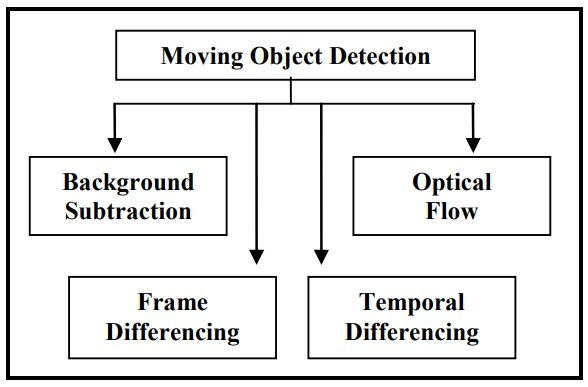
\includegraphics[width=8cm]{image/FourTraditionalMovingObjectDetection.jpg}
      \caption{Pendekatan Tradisional Deteksi Objek Bergerak}
      \small{Sumber: \citet{Kulchandani2015}}
      \label{fig:Pendekatan Tradisional Deteksi Objek Bergerak}
    \end{figure}
  
\section{\textit{Background Subtraction}}
    \textit{Background Subtraction} adalah metode yang digunakan untuk mendeteksi objek bergerak dalam video dengan cara membandingkan setiap \textit{frame} dengan sebuah \textit{(reference frame)} atau \textit{background model}, yang kemudian dihitung perbedaan nilai piksel diantara keduanya. Perbedaan inilah yang nantinya akan dikomparasi dengan sebuah \textit{threshold} yang nilainya sudah ditentukan. Jika perbedaan nilai piksel melebihi nilai \textit{threshold}, maka piksel tersebut dapat dikatakan bagian dari objek bergerak \textit{(foreground)} dan jika tidak, piksel akan dikatakan sebagai \textit{background} \citep{Desai2014}. Dalam banyak literasi, metode BS dapat dirumuskan sebagai berikut:
    \begin{equation}\label{eq:2.3}
    X_t (s) =
    \begin{cases} 
          1 &\text{\textit{if} $d(I_{s,t}, B_s) > T$}, \\
          0 &\text{\textit{otherwise}}
    \end{cases}
    \end{equation}
    
    Dimana $T$ adalah nilai \textit{threshold} yang sudah ditentukan, $X_t (s)$ adalah \textit{foreground mask} pada waktu $t$, $d$ adalah selisih antara $I_{s,t}$ yang merupakan nilai piksel $s$ pada waktu $t$, dengan $B_s$ yang merupakan \textit{background model} pada piksel $s$. Yang membedakan metode BS satu dengan yang lain biasanya terletak pada bagaimana metode tersebut memodelkan $B$ \citep{Benezeth2010}.
    
    \textit{Background modeling} adalah tahap yang penting dari \textit{Background Subtraction}. Objektif utama dari proses \textit{background modeling} adalah untuk mendapatkan model latar belakang yang berisikan informasi berupa bagian statis dari sebuah \textit{scene}, atau segala sesuatu yang dapat dikatakan sebagai latar belakang. Cara paling sederhana dalam memodelkan latar belakang $B$ adalah dengan sebuah citra yang berisikan \textit{scene} statis tanpa objek bergerak. Citra tersebut dapat diambil dari sebuah video ketika tidak ada objek yang bergerak di dalamnya.
    
    \vspace{0.5cm}
    \begin{figure}[H]
    \centering
      \singlespacing
      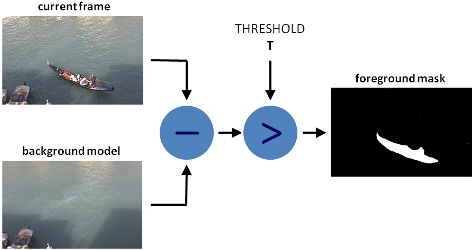
\includegraphics{image/BS.png}
      \caption{Skema sederhana metode \textit{Background Subtraction}}
      \small{Sumber: \href{https://docs.opencv.org/4.5.3/d1/dc5/tutorial_background_subtraction.html}{OpenCV - Background Subtraction}}
      \label{fig:BS}
    \end{figure}
    
    Dibalik kemudahan implementasinya, kelemahan dari metode tradisional ini adalah sistem tidak dapat mengatasi perubahan yang terjadi pada latar belakang selama video berlangsung. Karena dalam praktiknya, latar belakang sebuah video tidak akan selalu statis. Perubahan iluminasi, pergerakan berulang suatu objek (dahan pohon yang tertiup angin), atau perubahan bentuk geometri objek latar belakang tentu dapat memengaruhi akurasi metode ini.

\section{\textit{Background Subtraction} Menggunakan \textit{Gaussian Mixture Models}}
    \textit{Gaussian Mixture Models} (GMM) dapat digunakan untuk memodelkan latar belakang pada teknik \textit{Background Subtraction}. \citet{Stauffer1999}, dalam penelitiannya memodelkan sebuah piksel sebagai \textit{mixture of Gaussians}. Berdasarkan \textit{evidence} dan varians dari masing-masing distribusi Gaussian, dapat ditentukan distribusi mana yang masuk ke dalam kelas warna latar belakang \textit{(background color)}. Nilai piksel yang tidak masuk ke dalam distribusi warna latar belakang akan dianggap sebagai latar depan \textit{(foreground)} sampai ada distribusi Gaussian yang nilai piksel tersebut termasuk di dalamnya.
    
    Dikatakan oleh Stauffer bahwa sistem ini \textit{robust} terhadap latar belakang yang dinamis, seperti perubahan iluminasi, pergerakan berulang sebuah benda (dahan pohon yang tertiup angin), objek yang bergerak lambat, dan objek yang masuk serta keluar dari \textit{scene}. Objek yang bergerak lambat membutuhkan waktu yang lama untuk dapat dikatakan sebagai latar depan. Hal ini dikarenakan warna piksel mereka mempunyai varians yang lebih besar dibandingkan latar belakang. Sistem ini memiliki dua parameter, yaitu \textit{learning rate} $\alpha$ dan \textit{threshold} $T$ (proporsi data yang harus diperhitungkan/digunakan oleh latar belakang).
    
    \subsection{\textit{Gaussian Mixture Models}}
        Didefinisikan nilai sebuah piksel berturut-turut sebagai \textit{"pixel process"}. \textit{Pixel process} adalah serangkaian nilai piksel, nilai piksel tersebut dapat berupa skalar untuk citra \textit{grayscale} dan vektor untuk citra berwarna \textit{(r, g, b)}. Suatu hal yang dapat  diketahui dari sebuah piksel ${x_0, y_0}$ pada waktu $t$ adalah riwayat dari piksel itu sendiri.
        \begin{equation}\label{eq:2.4}
        \{X_1, \ldots, X_t\} = \{I(x_0, y_0, i) : 1 \leq i \leq t\}
        \end{equation}
        
        Dimana $I$ adalah serangkaian citra. Jika perubahan cahaya terjadi di dalam \textit{scene}, perubahan itu harus tetap dilacak oleh distribusi-distribusi Gaussian tersebut. Jika sebuah objek statis masuk ke dalam \textit{scene} dan tidak langsung masuk ke dalam distribusi latar belakang sampai objek tersebut sudah lebih lama ada di area tersebut dari objek sebelumnya, maka objek tersebut akan dikategorikan sebagai latar depan dalam waktu yang cukup lama. Hal ini akan berujung pada estimasi latar depan yang buruk. Misalnya dahan pohon yang bergerak karena tertiup angin, tentu tidak diinginkan objek tersebut dideteksi sebagai objek bergerak oleh sistem.
        
        Hal di atas adalah faktor yang menjadi landasan utama Stauffer dalam menentukan model dan prosedur updatenya. Riwayat dari setiap piksel $\{X_1, \ldots, X_t\}$ dimodelkan oleh $K$ distribusi Gaussian yang probabilitas nilai pikselnya didefinisikan oleh fungsi berikut
        
        \begin{equation}\label{eq:2.5}
        P(X_t) = \sum_{i=1}^K \omega_{i, t} \cdot \eta (X_t, \mu_{i, t}, \text{$\textstyle \sum$}_{i, t})
        \end{equation}
        
        Dimana $K$ adalah jumlah distribusi Gaussian, $\omega_{i, t}$ adalah estimasi dari \textit{evidence / weight / bobot} (proporsi data yang direpresentasikan oleh Gaussian yang bersangkutan), $\mu_{i, t}$ adalah nilai rata-rata dari Gaussian ke-$i$ pada waktu $t$, $\sum_{i, t}$ adalah kovarians matriks Gaussian ke-$i$ pada waktu $t$, dan $\eta$ adalah fungsi probabilitas Gaussian
        \begin{equation}\label{eq:2.6}
        \eta (X_t, \mu_t, \text{$\textstyle \sum$}) = 
        \frac{1}{{(2\pi)^\frac{n}{2} \textstyle |\sum|^\frac{1}{2} }}e^{ - \frac{1}{2} (X_t - \mu_t)^{T \sum{-1} } (X_t - \mu_t)}
        \end{equation}
        \vspace{0.005cm}
        
        Dengan kovarians matriks
        \begin{equation}\label{eq:2.7}
        \text{$\sum$}_{i, t} = \sigma^2_k I
        \end{equation}
        
        $K$ ditentukan oleh kemampuan komputasi komputer. Untuk nilai bawaan $K =  5$ diset dan dapat diatur sesuai dengan kebutuhan pengguna untuk mendapatkan hasil terbaik.
        
    \subsection{\textit{Modeling Process}}
        Distribusi intensitas untuk setiap nilai piksel dimodelkan oleh \textit{mixture of Gaussian}. Secara garis besar, jika ada nilai piksel baru yang masuk ke dalam model, piksel tersebut akan direpresentasikan oleh salah satu komponen atau distribusi Gaussian yang ada dan digunakan untuk memperbarui model tersebut. Teknik \textit{on-line K-means approximation} digunakan untuk memodelkan distribusi nilai masing-masing piksel.
        
        Langkah pertama yang harus dilakukan adalah, inisialisasi Gaussian $\eta$ untuk memodelkan nilai piksel pada observasi $X_1$ dengan $\omega = 1$, $\mu = X_1$, dan varians $\sigma$ yang besar. Observasi $X_1$ adalah observasi nilai sebuah piksel pada waktu $t$. Selanjutnya, setiap piksel baru $X_t$ diperiksa terhadap $K$ distribusi Gaussian yang sudah ada, sampai terdapat \textit{"match"}. Sebuah nilai piksel dapat dikatakan \textit{"match"} dengan $K$ distribusi Gaussian jika nilai piksel terletak dalam jangkauan 2,5 dari standar deviasi distribusi tersebut. Jika terdapat \textit{"match"}, parameter $(\omega, \mu, \sigma)$ dari distribusi Gaussian diperbarui sebagai berikut
        \begin{equation}\label{eq:2.8}
        \omega_{k, t} = (1 - \alpha)\omega_{k, t-1} + \omega(M_{k, t})
        \end{equation}
        \begin{equation}\label{eq:2.9}
        \mu_t = (1 - \rho)\mu_t-1 + \rho X_t
        \end{equation}
        \begin{equation}\label{eq:2.10}
        \sigma^2_t = (1 - \rho)\sigma^2_t-1 + \rho (X_t - \mu_t)^T (X_t - \mu_t)
        \end{equation}
        \vspace{0.005cm}
        
        Dimana $\alpha$ adalah \textit{learning rate}, $M_{k, t}$ bernilai 1 untuk distribusi yang \textit{"matched"}, dan 0 untuk distribusi yang lainnya. Lalu
        \begin{equation}\label{eq:2.11}
        \rho = \alpha\eta(X_t|\mu_t, \sigma_t)
        \end{equation}
        
        Jika tidak ada distribusi $K$ yang \textit{"match"} dengan nilai piksel baru tersebut, maka buat distribusi baru yang menggunakan nilai piksel baru sebagai rata-ratanya, nilai varians awal yang besar, dan juga bobot yang rendah. Distribusi yang paling kecil kemungkinannya akan digantikan oleh distribusi baru jika $K \text{\textit{Gaussians}} > K$.
        
    \subsection{\textit{Background Model Estimation}}
        Dalam tahap ini, ditentukan distribusi Gaussian mana yang merupakan bagian dari latar belakang. Secara heuristik, distribusi Gaussian yang memiliki bobot yang paling tinggi dan juga varians yang paling kecil adalah distribusi yang dapat diklasifikasikan sebagai latar belakang. Untuk memahami hal tersebut, diberikan sebuah objek statis yang mempunyai distribusi nilai piksel dengan bobot yang tinggi dan juga varians yang kecil. Objek statis ini dapat dikatakan sebagai \textit{background} dalam suatu \textit{scene} video. Ketika terdapat objek baru yang melewati objek statis tersebut, nilai piksel objek baru tidak akan \textit{"match"} dengan salah satu distribusi Gaussian yang sudah ada sebelumnya. Hal ini akan berujung pada pembuatan distribusi baru atau peningkatan nilai varians dari distribusi yang sudah ada. Selain itu, varians dari objek bergerak diasumsikan bernilai lebih besar daripada varians latar belakang. Untuk memodelkan hal tersebut, dibutuhkan sebuah metode yang dapat menentukan bagian mana dari model distribusi Gaussian yang secara akurat merepresentasikan latar belakang.
        
        Pertama, distribusi Gaussian diurutkan berdasarkan nilai $\omega/\sigma$ dari masing-masing distribusi. Kemudian, \textit{background model} dipilih berdasarkan fungsi berikut, dimana $T$ adalah sebuah ukuran untuk menentukan seberapa besar bagian dari data yang dapat diklasifikasikan sebagai latar belakang.
        \begin{equation}\label{eq:2.12}
        B = argmin_b (\sum_{k=1, b}\omega_k > T)
        \end{equation}
        
        
\section{Operasi Morfologi}
    Morfologi dalam konteks pengolahan citra adalah deskripsi bentuk dan struktur dari sebuah objek di dalam citra. Berdasarkan hal tersebut, operasi morfologi adalah sebuah operasi yang diaplikasikan terhadap bentuk dan struktur sebuah objek di dalam citra. Teknik ini bekerja berdasarkan teori himpunan. Operasi Morfologi mengambil input berupa citra biner ataupun citra \textit{grayscale} \citep{Srisha2013}. Operasi Morfologi dapat digunakan untuk memperbesar atau memperkecil ukuran objek. Operasi morfologi juga dapat digunakan untuk menutup ataupun membuka lubang pada sebuah objek dalam citra.
    
    Operasi morfologi melakukan "pemindaian" terhadap sebuah citra dengan menggunakan \textit{Structuring element}. \textit{Structuring element} adalah sebuah matriks biner yang biasanya direpresentasikan sebagai matriks persegi berdimensi ganjil. Mekanisme pemindaian citra menggunakan \textit{structuring element} sangat menyerupai \textit{kernel / mask} pada operasi konvolusi. Akan tetapi, alih-alih melakukan operasi konvolusi, \textit{structuring element} hanya melakukan operasi logika sederhana. Interaksi antara \textit{structuring element} dengan citra yang ingin diperiksa akan menghasilkan citra baru berdasarkan jenis operasi morfologi yang diterapkan pada citra tersebut.
    \begin{figure}[H]
    \centering
      \singlespacing
      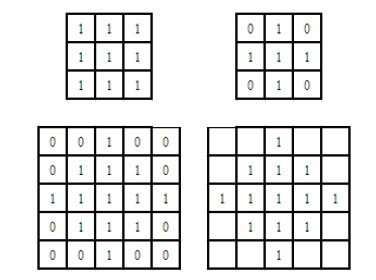
\includegraphics{image/StructuringElement.jpg}
      \caption{Representasi \textit{Structuring Element}}
      \small{Sumber: \citet{Srisha2013}}
      \label{fig:SS}
    \end{figure}
    
\section{Jenis - Jenis Operasi Morfologi}
    Walaupun operasi morfologi berdasar pada teori himpunan, banyak dari jenis operasi ini yang secara garis besar hanyalah operasi logika sederhana dan sangat mudah untuk digunakan. Terdapat dua jenis operasi fundamental dari operasi morfologi, yaitu erosi dan dilasi. Jenis operasi yang lain sangat bergantung kepada dua operasi fundamental tersebut.\\\\
    
    \subsection{Erosi}
        Operasi erosi membuat objek pada citra menjadi lebih kecil. Sederhananya, piksel di sekitar garis tepi sebuah objek akan dihilangkan. Erosi dapat digunakan untuk menghilangkan \textit{noise} pada citra dan juga memisahkan objek satu dengan yang lainnya. Erosi dari sebuah citra $A$ oleh \textit{structuring element} $B$ dapat didefinisikan oleh fungsi berikut
        \begin{equation}\label{eq:2.13}
        A \ominus B = \{z | (B)_z \subseteq A\}
        \end{equation}
        
        \textit{Structuring element} yang sudah dibuat akan memindai seluruh piksel di dalam citra dari mulai kiri ke kanan, dan dari atas ke bawah. Sebuah piksel tengah dari \textit{structuring element} akan dibiarkan bernilai 1 jika seluruh piksel di dalam \textit{structuring element} bernilai 1. Jika tidak, piksel akan dihilangkan atau diset nilainya menjadi 0 \textit{(background)}.
        \begin{figure}[H]
        \centering
          \singlespacing
          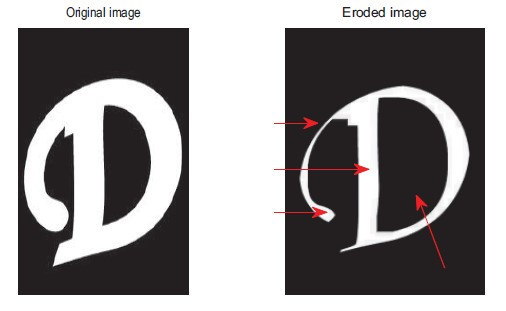
\includegraphics[width=10cm]{image/erosi.jpg}
          \caption{Operasi Erosi}
          \small{Sumber: \citet{Srisha2013}}
          \label{fig:Erosi}
        \end{figure}
    
    \subsection{Dilasi}
        Operasi dilasi membuat objek pada citra bertambah ukurannya menjadi lebih besar. Seberapa jauh operasi ini dapat membuat objek menjadi lebih besar bergantung pada bentuk dan ukuran \textit{structuring element}-nya. Dilasi sangat berguna untuk menutup lubang pada objek atau menggabungkan bagian-bagian objek yang terpisah. Operasi ini dapat didefinisikan sebagai
        \begin{equation}\label{eq:2.14}
        A \oplus B = \{z | \widehat{(B)_z} \cap A \neq \emptyset\}
        \end{equation}
        
        Sama seperti erosi, dilasi juga menggunakan \textit{structuring element} dalam proses pemindaian citra. Sebuah piksel tengah dari \textit{structuring element} diset nilainya menjadi 1 jika  \textit{structuring element} memiliki paling tidak satu piksel yang bernilai 1.
        \begin{figure}[H]
        \centering
          \singlespacing
          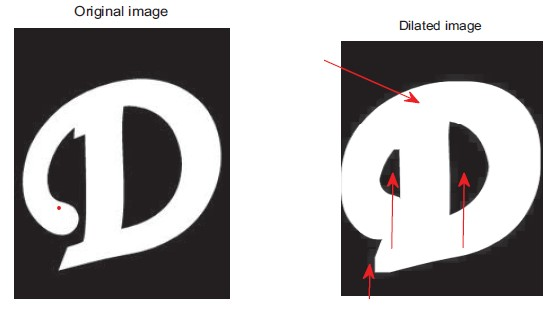
\includegraphics[width=12cm]{image/dilasi.jpg}
          \caption{Operasi Dilasi}
          \small{Sumber: \citet{Srisha2013}}
          \label{fig:Dilasi}
        \end{figure}
    
    \subsection{\textit{Opening}}
        \textit{Opening} adalah erosi yang diikuti oleh dilasi. Jenis operasi ini sangat berguna untuk menghilangkan objek yang sangat kecil atau \textit{noise} pada citra. \textit{Opening} citra $A$ oleh \textit{structuring element} $B$ dapat didefinisikan sebagai
        \begin{equation}\label{eq:2.15}
        A \text{ $o$ } B = (A \ominus B) \oplus B
        \end{equation}
        \begin{figure}[H]
        \centering
          \singlespacing
          
\includegraphics[width=8cm]{image/opening.jpg}
          \caption{Operasi \textit{Opening}}
          \small{Sumber: \href{https://docs.opencv.org/3.4.15/d3/dbe/tutorial_opening_closing_hats.html}{OpenCV - Opening}}
          \label{fig:Opening}
        \end{figure}
    
    \subsection{\textit{Closing}}
        \textit{Closing} adalah kebalikan dari operasi \textit{opening}. \textit{Closing} adalah dilasi yang diikuti oleh erosi. Seperti namanya, operasi \textit{closing} digunakan untuk menutup lubang di dalam sebuah objek atau menyambungkan bagian-bagian objek yang terpisah. \textit{Closing} citra $A$ oleh \textit{structuring element} $B$ dapat didefinisikan sebagai
        \begin{equation}\label{eq:2.16}
        A \text{ $o$ } B = (A \oplus B) \ominus B
        \end{equation}
        \begin{figure}[H]
        \centering
          \singlespacing
          
\includegraphics[width=8cm]{image/closing.jpg}
          \caption{Operasi \textit{Closing}}
          \small{Sumber: \href{https://docs.opencv.org/3.4.15/d3/dbe/tutorial_opening_closing_hats.html}{OpenCV - Closing}}
          \label{fig:Closing}
        \end{figure}

\section{\textit{Downsampling}}
    \textit{Downsampling} merupakan salah satu operasi fundamental yang sering digunakan dalam pengolahan citra. \textit{Downsampling} adalah proses mereduksi resolusi spasial dari sebuah citra dengan tetap mempertahankan representasi 2D dari citra tersebut. Operasi ini biasanya digunakan untuk mengurangi ukuran penyimpanan dari sebuah citra. Beberapa metode standar untuk melakukan operasi ini diantaranya adalah \textit{decimation} dan \textit{averaging}.

    \textit{Decimation} adalah proses mengeliminasi piksel dari sebuah citra. Terdapat beberapa \textit{pattern} yang biasa digunakan, seperti menghapus setiap baris dan kolom piksel yang bernomor genap. Metode lainnya adalah \textit{averaging}, yang menggabungkan beberapa piksel menjadi satu buah piksel dengan cara \textit{averaging} (dicari rata-ratanya).
    \begin{figure}[H]
    \centering
      \singlespacing
      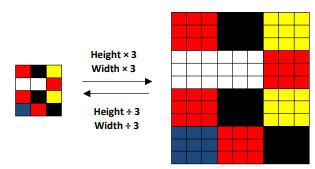
\includegraphics[width=7cm]{image/upsampling and downsampling.png}
      \caption{\textit{Image Downsampling dan Upsampling}}
      \small{Sumber: \citet{Paul2021}}
      \label{fig:Image Downsampling and Upsampling}
    \end{figure}
    \begin{figure}[H]
    \centering
      \singlespacing
      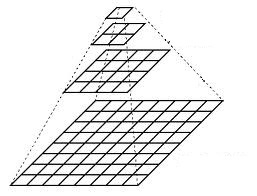
\includegraphics[width=5cm]{image/Pyramids_Tutorial_Pyramid_Theory.png}
      \caption{Piramid Citra}
      \small{Sumber: \href{https://docs.opencv.org/3.4/d4/d1f/tutorial_pyramids.html}{OpenCV - Image Pyramid}}
      \label{fig:Piramid Citra}
    \end{figure}

  
\section{Contour Tracing}
    \textit{Contour Tracing} atau \textit{Border Following} adalah salah satu teknik yang sangat penting dalam bidang pengolahan citra digital, terutama pada citra biner. \textit{Border following} telah dipelajari secara mendalam karena metode ini memiliki jangkauan pengaplikasian yang sangat luas, seperti pengenalan objek, analisis citra, deteksi objek, dan kompresi data citra \citep{Suzuki1985}.
    
    \citet{Suzuki1985} dalam penelitiannya menawarkan dua buah algoritme \textit{border following} yang sampai saat ini masih banyak digunakan oleh berbagai macam \textit{library} pengolahan citra modern seperti OpenCV. Algoritme ini adalah salah satu algoritme yang pertama kali mendefinisikan hubungan hierarki antar tepi \textit{(border)}. Selain itu, algoritme ini juga dapat membedakan tepi luar \textit{(outer border)} dan tepi lubang \textit{(hole border)} di sebuah objek. Beberapa definisi yang terdapat pada algoritme ini antara lain:
    
    \begin{itemize}
        \item \textbf{Definisi 1 (\textit{border point})}. Sebuah piksel bernilai 1 yang dikelilingi oleh piksel bernilai 0 dapat disebut sebagai \textit{border point}.
        \item \textbf{Definisi 2 (komponen yang mengelilingi komponen lain)}. Dari Gambar \ref{fig:Hubungan-antar-komponen-dan-tepi} dapat dikatakan bahwa komponen $S_2$ mengelilingi komponen $S_4$.
        \item \textbf{Definisi 3 (\textit{outer border} dan  \textit{hole border})}. Sebuah rangkaian \textit{border point} antara komponen yang mempunyai nilai piksel 1 (objek) dengan komponen yang mempunyai nilai piksel 0 (latar belakang).
        \item \textbf{Definisi 4 (\textit{parent border})}. Dari Gambar \ref{fig:Hubungan-antar-komponen-dan-tepi} dapat dikatakan bahwa tepi $B_2$ adalah \textit{parent border} dari tepi $B_3$.
        \item \textbf{Definisi 5 (tepian yang mengelilingi tepian lain)}. Dari Gambar \ref{fig:Hubungan-antar-komponen-dan-tepi} dapat dikatakan bahwa tepi $B_2$ mengelilingi tepi $B_3$.
    \end{itemize}
    \begin{figure}[H]
    \centering
      \singlespacing
      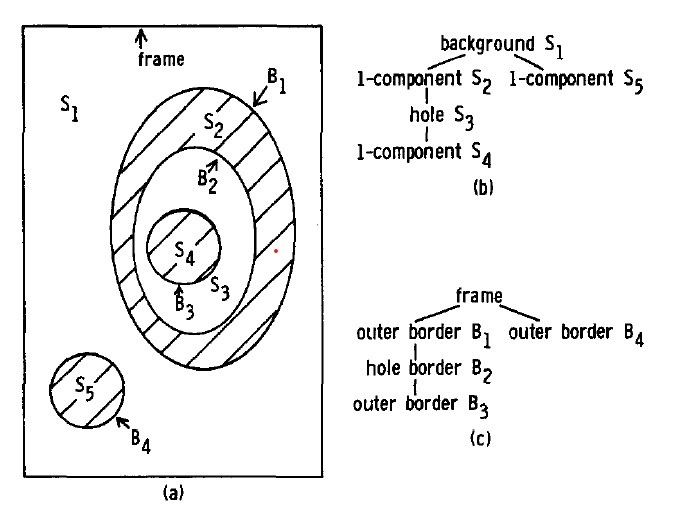
\includegraphics[width=10cm]{image/surroundess.jpg}
      \caption{Hubungan antar komponen dan tepi}
      \small{Sumber: \citep{Suzuki1985}}
      \label{fig:Hubungan-antar-komponen-dan-tepi}
    \end{figure}
    
    Diasumsikan citra masukan algoritme ini berupa citra biner. Piksel dengan nilai 0 dan 1 disebut sebagai 0-piksel dan 1-piksel. Piksel bernilai 0 merepresentasikan latar belakang, sementara piksel bernilai 1 merepresentasikan latar depan (objek). Didefinisikan $f_{i, j}$ sebagai nilai sebuah piksel pada koordinat $(i, j)$ yang masing-masing melambangkan baris dan kolom sebuah citra digital. Baris paling atas, baris paling bawah, kolom paling kiri, dan kolom paling kanan adalah \textit{frame} dari citra tersebut. Dalam hal ini, diberikan angka unik untuk setiap tepi baru yang ditemukan dan bisa disebut sebagai \textbf{NBD}. Asumsikan NBD dari \textit{frame} adalah 1, sementara tepi lain diberikan angka NBD secara berurutan. Nilai NBD dari \textit{parent} setiap tepi di dalam variabel \textbf{LNBD} kemudian disimpan. Berikut adalah langkah-langkah \textit{border following} algoritme 1:
    
    Mulai memindai piksel citra dari kiri ke kanan hingga \textit{scanner} menemukan piksel objek $f_{i, j} \neq 0$. Lalu tentukan apakah piksel tersebut merupakan tepi luar atau tepi lubang. Untuk setiap baris baru yang dipindai, \textit{reset} $LNBD$ ke 1.\\\\
    
    \begin{enumerate}
        \item Langkah 1
        
        \begin{enumerate}[label=(\alph*)]
            \item Jika $f_{i, j} = 1$ dan $f_{i, j - 1} = 0$, maka piksel $(i, j)$ adalah \textit{starting point} dari operasi \textit{border following} untuk tepi luar \textit{(outer border)}. Inkremen $NBD$ dan set $(i_2, j_2) \leftarrow (i, j-1)$.
            \item Jika $f_{i, j} \geq 1$ dan $f_{i, j+} = 0$, maka piksel $(i, j)$ adalah \textit{starting point} dari operasi \textit{border following} untuk tepi lubang \textit{(hole border)}. Inkremen $NBD$, set $(i_2, j_2) \leftarrow (i, j + 1)$, dan $LNBD \leftarrow f_{i, j}$ jika $f_{i, j} > 1$.
            \item Jika dua kondisi di atas tidak terpenuhi, maka lanjutkan ke langkah 4.
        \end{enumerate}
        
        \vspace{-0.9cm}
        \begin{figure}[H]
        \centering
          \singlespacing
          \captionsetup{justification=centering,margin=2cm}
          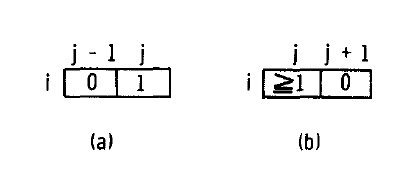
\includegraphics[width=6cm]{image/outerorholeborder.jpg}
          \caption{Kondisi \textit{starting point} dari algoritme \textit{border following} untuk tepi luar (a) dan tepi lubang (b)}
          \small{Sumber: \citep{Suzuki1985}}
          \label{fig:outerandholeborder}
        \end{figure}
        
        \item Langkah 2
        
        Berdasarkan jenis tepi dari piksel $(i, j)$ dan jenis tepi dari $LNBD$ (tepi terakhir yang ditemukan), dapat ditentukan \textit{parent border} untuk tepi piksel $(i, j)$ seperti yang terlihat pada Tabel \ref{tab:parentborder}.
    
    	\vspace{3cm}
	    \begin{longtblr}[
	    	caption = {Aturan penetapan \textit{parent border}},
	    	label = {tab:parentborder}
	    	]{
	    		colspec={|c|Q[c,m,4.5cm]|Q[c,m,4.5cm]|},
	    		rowhead=1
	    	}
	    	\hline
	    	& \SetCell[c=2]{} \textit{Type of the border B' with the sequential number LNBD} \\ \hline
	    	\textit{Type of B} & \textit{Outer border} & \textit{Hole border} \\ \hline
	    	\textit{Outer border} & \textit{The parent border of the border B'} & \textit{The border B'} \\ 
	    	\textit{Hole border} & \textit{The border B'} & \textit{The parent border of the border B'} \\ 
	    	\hline
	    \end{longtblr}
        
        \item Langkah 3
        
        Pada langkah ini, dimulai dari \textit{starting point} piksel $(i, j)$ lakukan proses \textit{border following}:
        \begin{enumerate}
            \item Dimulai dari piksel $(i_2, j_2)$, searah jarum jam periksa piksel tetangga dari piksel $(i, j)$ sampai menemukan piksel \textit{non-zero}. Didefinisikan piksel \textit{non-zero} yang pertama ditemukan sebagai $(i_1, j_1)$. Jika piksel \textit{non-zero} tidak ditemukan, set $f_{i, j} = -NBD$ dan lanjutkan ke langkah 4.
            
            \item $(i_2, j_2) \leftarrow (i_1, j_1)$ dan $(i_3, j_3) \leftarrow (i, j)$.
            
            \item Mulai dari elemen selanjutnya dari piksel $(i_2, j_2)$, berlawanan arah jarum jam carilah piksel \textit{non-zero} di sekitar piksel $(i_3, j_3)$ dan set piksel $non-zero$ pertama yang ditemukan tersebut ke dalam variabel $(i_4, j_4)$.
            
            \item Ubah nilai $f_{i_3, j_3}$ dari piksel $(i_3, j_3)$ seperti berikut \textit{marking policy}:
            \begin{enumerate}
                \item Jika piksel $(i_3, j_3 + 1)$ dari langkah (3.a) adalah 0-piksel (piksel bernilai 0), set $(i_3, j_3 + 1) \leftarrow -NBD$
                \item Jika piksel $(i_3, j_3 + 1)$ dari langkah (3.a) bukan 0-piksel (piksel bernilai 0), set $(i_3, j_3 + 1) \leftarrow NBD$
                \item Jika kedua kondisi di atas tidak terpenuhi, jangan ubah nilai  $f_{i_3, j_3}$
            \end{enumerate}
            
            \item Jika  $(i_4, j_4) = (i, j)$ dan $(i_3, j_3) = (i_1, j_1)$ (kembali ke \textit{starting point}), maka lanjut ke langkah 4, Jika tidak set $(i_2, j_2) \leftarrow (i_3, j_3)$, $(i_3, j_3) \leftarrow (i_4, j_4)$ dan kembali ke langkah (3.a).
        \end{enumerate}
        
        \item Langkah 4
        
        Jika $f_{i, j} \neq 1$, maka $LNBD \leftarrow |f_{i, j}|$ dan lanjutkan pemindaian dari mulai piksel $(i, j+1)$ untuk kembali mencari nilai piksel objek $f_{i, j} \neq 0$. Alrogritme dinyatakan selesai jika \textit{scanner} sudah sampai sudut kanan bawah dari citra  tersebut (piksel terakhir).
        
        \begin{figure}[H]
        \centering
          \singlespacing
          \captionsetup{justification=centering,margin=0.5cm}
          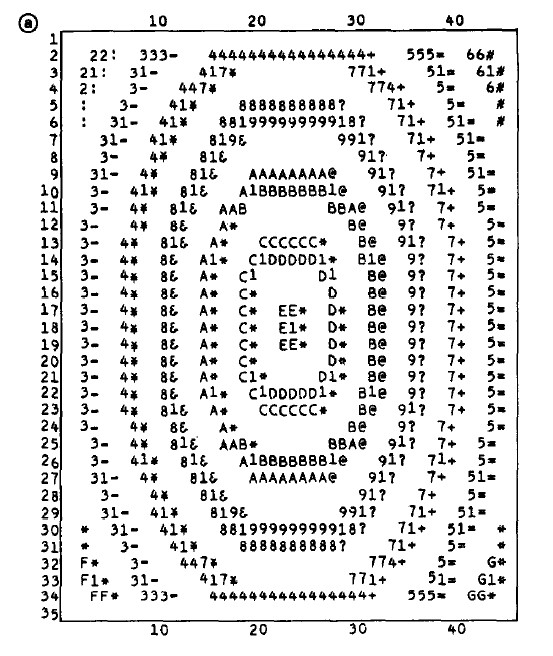
\includegraphics[width=8cm]{image/topologicalresult.jpg}
          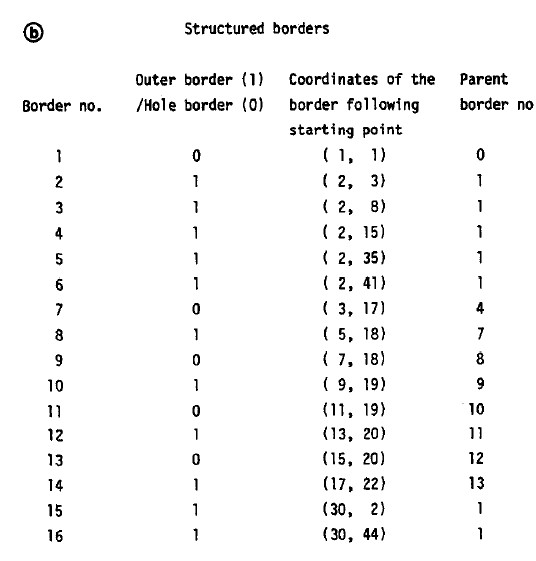
\includegraphics[width=10cm]{image/topologicalstructure.jpg}
          \caption{Struktur topologi antara tepi satu dengan tepi yang lain jika menggunakan Algoritme 1. Hasil citra (a) dan Struktur yang diekstrak (b)}
          \small{Sumber: \citep{Suzuki1985}}
          \label{fig:parentborder}
        \end{figure}
    \end{enumerate}
    
    Selain algoritme di atas, Suzuki juga mengusulkan algoritme \textit{border following} yang hanya akan menghasilkan tepi terluarnya saja. Beberapa perbedaan algoritme 1 dan algoritme 2 antara lain adalah:
    
    \begin{enumerate}
        \item Kondisi \textit{starting point} untuk melakukan operasi \textit{border following} hanya berlaku untuk tepi terluar (Gambar \ref{fig:outerandholeborder}) dan jika $LNBD \leq 0$.
        \item \textit{Marking policy} tetap sama dengan algoritme 1 (Langkah 3.d), tetapi nilai dari $NBD$ dan $-NBD$ akan digantikan masing-masing oleh nilai $2$ dan  $-2$.
        \item Nilai $LNBD$ juga tetap disimpan dari piksel \textit{non-zero} yang ditemukan sebelumnya. Akan tetapi, $LNBD$ akan di reset ke nilai 0 untuk setiap baris baru yang dipindai.
    \end{enumerate}
    \vspace{-0.9cm}
    \begin{figure}[H]
    \centering
      \singlespacing
      \captionsetup{justification=centering,margin=0.5cm}
      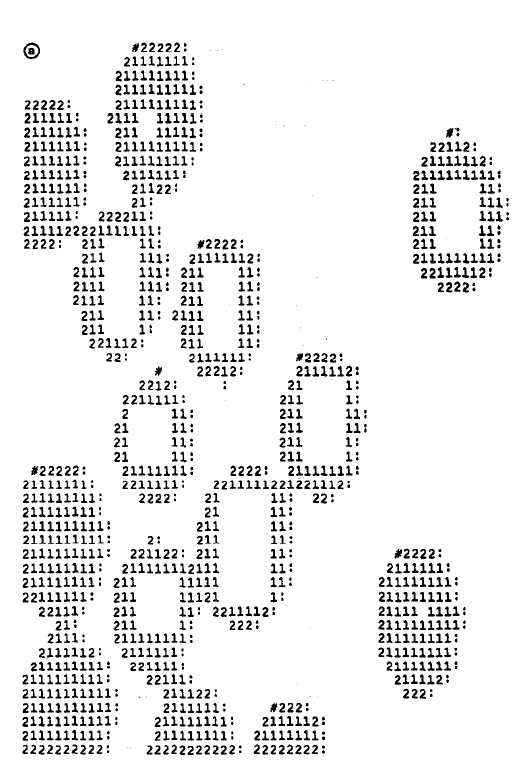
\includegraphics[width=8.1cm]{image/algoritma2.jpg}
      \caption{Hasil dari algoritme 2. Tanda "\#" merepresentasikan \textit{starting point} dan ":" merepresentasikan nilai $-2$}
      \small{Sumber: \citep{Suzuki1985}}
      \label{fig:parentborder}
    \end{figure}
    
\section{Pelacakan Objek}
    Pelacakan objek \textit{(object tracking)} mengacu kepada penggunaan sensor untuk menentukan lokasi, lintasan, atau bahkan karakteristik dari sebuah objek. Dalam kasus video, pelacakan objek didefinisikan sebagai sebuah tindakan melakukan estimasi atau prediksi terhadap lintasan sebuah objek bergerak di setiap \textit{frame} dalam video. Dengan kata lain, sebuah \textit{tracker} dapat memberikan label / identitas yang konsisten terhadap objek yang dilacak selama video berlangsung. Selain itu, sebuah \textit{tracker} juga dapat memberikan informasi lain yang berkaitan dengan objek tersebut, seperti orientasi, ukuran, atau bentuk geometrinya \citep{Yilmaz2006}.
    
    Permintaan terhadap teknologi analisis video yang lebih \textit{advanced} membuat metode pelacakan objek menjadi sangat menarik untuk dikembangkan. Penggunaan metode pelacakan objek sangat berguna dalam berbagai bidang, antara lain seperti \textit{motion recognition}, pengawasan, pemantauan lalu lintas, navigasi kendaraan, dan masih banyak lagi. Pelacakan objek merupakan dasar teori dari metode penghitungan objek \textit{(objek counting)}.
  
\section{Kalman Filter}

    \subsection{Definisi}
        Secara matematis, Kalman Filter adalah sebuah algoritme \textit{estimator} yang dapat melakukan prediksi dan koreksi terhadap keadaan sebuah proses linear \citep{Chavan2017}. Model matematis yang akurat sangat diperlukan untuk mendapatkan hasil yang optimal. Kalman Filter memiliki bentuk yang relatif sederhana dan tidak membutuhkan kekuatan komputasi yang besar.
        
        Kalman filter digunakan untuk melakukan estimasi suatu keadaan $x$ dalam sistem linear. Model dari proses \textit{(process model)} yang mendefinisikan evolusi suatu keadaan dari waktu $k - 1$ sampai waktu $k$ adalah:
        \begin{equation}\label{eq:2.17}
        x_k = Fx_{k-1} + Bu_{k-1} + w_{k-1} 
        \end{equation}
        
        dimana $F$ adalah matriks transisi dari keadaan $x$ yang diterapkan pada vektor keadaan sebelumnya $x_{k-1}$, $B$ adalah matriks kontrol yang diterapkan pada vektor kontrol $u_{k-1}$, dan $w_{k-1}$ adalah vektor proses \textit{noise} yang diasumsikan sebagai Gaussian dengan rata-rata nol dan kovarians $Q$, i.e., $w_{k-1} \sim N(0, Q)$.
        
        Model proses di atas dipasangkan dengan model pengukuran / observasi \textit{(measurement / observation model)} yang menggambarkan hubungan antara keadaan dan observasi pada waktu $k$ sebagai:
        \begin{equation}\label{eq:2.18}
        z_k = Hx_{k} + v_{k} 
        \end{equation}
        
        dimana $z_k$ adalah vektor observasinya, H adalah matriks transisi dari observasi $z$, dan $v_{k}$ adalah vektor \textit{noise} dari observasi yang diasumsikan sebagai Gaussian dengan rata-rata nol dan kovarians $R$, i.e., $v_{k} \sim N(0, R)$.
        
        Peran dari Kalman Filter adalah untuk memberikan estimasi $x$ pada waktu $k$, mengingat diberikannya estimasi awal $x_0$, rangkaian observasi $z1, z1, ..., zk$, dan informasi sistem yang digambarkan oleh $F$, $B$, $H$, $Q$, dan $R$. Walaupun matriks kovarians ($Q$ dan $R$) seharusnya mencerminkan statistik dari \textit{noise} masing-masing model, dalam banyak pengaplikasiannya di dunia nyata, model statistika dari \textit{noise} tersebut tidak benar-benar dapat dimodelkan. Karena hal itu, $Q$ dan $R$ biasanya digunakan sebagai \textit{tuning parameter} yang bisa digunakan untuk mendapatkan hasil dan performa yang diinginkan.
    
    \subsection{Algoritme Kalman Filter}
        Kalman Filter terdiri dari dua tahap, yaitu \textit{predict} dan \textit{update}. Dalam literasi lain, tahapan ini juga biasa disebut sebagai \textit{propagation} dan \textit{correction}. Tahapan \textit{predict} dan \textit{update} dapat diringkas ke dalam persamaan berikut:\\\\
        
        \noindent\textit{Predict}
        \begin{equation}\label{eq:2.19}
        \hat{x}^-_k = F\hat{x}^+_{k-1} + Bu_{k-1}
        \end{equation}
        \begin{equation}\label{eq:2.20}
        P^-_k = FP^+_{k-1}F^T + Q
        \end{equation}
        \textit{Update}
        \begin{equation}\label{eq:2.21}
        \tilde{y}_k = z_k - H\hat{x}^-_k
        \end{equation}
        \begin{equation}\label{eq:2.22}
        K_k = P^-_kH^T(R + HP^-_kH^T)^{-1}
        \end{equation}
        \begin{equation}\label{eq:2.23}
        \hat{x}^+_k = \hat{x}^-_k + K_k\tilde{y}
        \end{equation}
        \begin{equation}\label{eq:2.24}
        P^+_k = (I - K_kH)P^-_k
        \end{equation}
        
        Dari persamaan di atas, operator hat ($\string^$) menandakan sebuah estimasi dari sebuah variabel. Dengan kata lain, $\hat{x}$ adalah estimasi dari $x$. Superskrip $-$ dan $+$ masing-masing menyatakan estimasi yang diprediksi \textit{(prior)} dan diperbarui \textit{(posterior)}.
        
        Untuk memprediksi estimasi dari sebuah keadaan $\hat{x}^-_k$ dibutuhkan estimasi keadaan $\hat{x}^+_{k-1}$ dari iterasi Kalman Filter sebelumnya. Variabel $P$ adalah matriks kovarians dari keadaan $x$. Matriks kovarians ini digunakan untuk membantu Kalman Gain $K_k$ dalam menentukan bobot terhadap nilai yang diprediksi atau nilai yang diukur.
        
        Dalam tahap \textit{update}, $K_k$ pada Persamaan \ref{eq:2.22} adalah Kalman Gain. Nilai dari Kalman Gain akan berada diantara 0 dan 1. Kemudian nilai tersebut digunakan untuk memperbarui estimasi keadaan $\hat{x}^+_k$. Jika nilai dari Kalman Gain mendekati 1, maka observasi dikatakan akurat dan estimasi dikatakan tidak akurat (\textit{error} besar). Begitu juga sebaliknya, jika $K_k$ mendekati 0, maka observasi dikatakan tidak akurat dan estimasi dapat dikatakan akurat (\textit{error} kecil). Akibatnya, nilai $K_k$ yang kecil akan membuat selisih antara keadaan yang diobservasi dan keadaan yang diestimasi mempunyai efek yang kecil terhadap proses pembaruan keadaan (Persamaan \ref{eq:2.23}). Residual pengukuran $\tilde{y}_k$ adalah selisih antara nilai yang diobservasi $z_k$, dengan nilai yang diestimasi $H\hat{x}^-_k$. Residual pengukuran $\tilde{y}_k$ kemudian dikalikan dengan Kalman Gain $K_k$ untuk memberikan koreksi $K_k\tilde{y}_k$ terhadap estimasi keadaan $\hat{x}^-_k$ (Persamaan \ref{eq:2.23}). Setelah mendapatkan estimasi keadaan yang baru, Kalman Filter menghitung kovarians $P^+_k$ untuk kemudian digunakan pada tahap atau iterasi Kalman Filter selanjutnya. Dapat dilihat bahwa kovarians $P^+_k$ mempunyai nilai yang lebih kecil dibandingkan kovarians $P^-_k$, yang berarti Kalman Filter menjadi lebih yakin dengan estimasi keadaan setelah tahap \textit{update}.
        
        Dibutuhkan tahap inisialisasi untuk dapat mengimplementasi Kalman Filter. Dalam tahap tersebut, dibutuhkan tebakan awal dari $\hat{x}^+_0$ dan juga matriks kovarians $P^+_0$. Bersama dengan $Q$ dan $R$, $\hat{x}^+_0$ dan $P^+_0$ memainkan peran yang sangat penting untuk mendapatkan hasil dan performa yang diinginkan. Sebagai \textit{"rule of thumb"}, kovarians $P^+_0$ dapat diset ke nilai yang besar untuk konvergensi yang lebih cepat. Secara keseluruhan, Kalman Filter dapat diimplementasi dengan menerapkan tahap \textit{predict} dan tahap \textit{update} untuk setiap iterasi waktu $k = 1, 2, 3, ...$ setelah tahap inisialisasi dilakukan.
        
        Perlu dicatat bahwa Kalman Filter bekerja berdasarkan asumsi bahwa model proses \textit{(process model)} dan model pengukuran \textit{(measurement model)} merupakan model yang linear, yang berarti model-model tersebut dapat diekspresikan dengan matriks F, B, dan H. Oleh karena itu, Kalman Filter dapat memberikan hasil estimasi yang optimal jika dan hanya jika asumsi di atas terpenuhi.
        
\section{\textit{Decision of Occlusion}}
    \textit{Occlusion} adalah sebuah peristiwa dimana dua atau lebih objek saling bertumpuk satu sama lain. Hal ini tentu dapat berpengaruh terhadap performa sistem jika tidak ditangani dengan baik. \textit{Occlusion} pada dasarnya mencakup dua masalah, yaitu masalah \textit{merge} dan \textit{split}. Menyatunya dua atau lebih objek disebut sebagai proses \textit{merge}. Sebaliknya, terpisahnya objek yang sebelumnya menyatu disebut sebagai proses \textit{split}. Proses \textit{merge} dan \textit{split} diilustrasikan pada Gambar \ref{fig:mergesplit}.
    \begin{figure}[H]
    \centering
      \singlespacing
      \captionsetup{justification=centering,margin=0.5cm}
      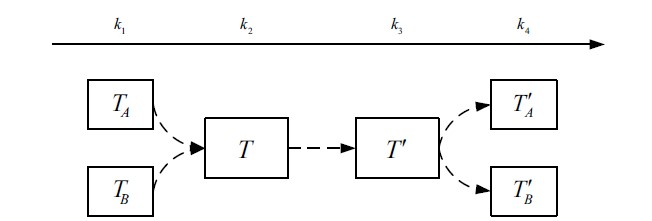
\includegraphics[width=12cm]{image/mergesplit-02.jpg}
      \caption{Ilustrasi dari proses \textit{merge} dan \textit{split}}
      \small{Sumber: \citep{Li2010}}
      \label{fig:mergesplit}
    \end{figure}
    
    Ketika dua atau lebih keadaan objek yang diprediksi menggunakan Kalman Filter mempunyai pasangan observasi (deteksi) yang sama, maka akan terjadi proses \textit{merge} sebagai bagian dari salah satu proses \textit{decision of occlusion}. Dua buah objek $T_A$ dan $T_B$ mengalami proses \textit{merge} pada waktu $k_1$. Dimulai dari waktu $k_2$, objek $T$ akan dilacak sebagai objek baru, Kalman Filter diinisialisasi untuk objek tersebut. Selama waktu $k_2$ sampai $k_3$, objek $T$ akan terus diupdate bersamaan dengan objek $T_A$ dan objek $T_B$. Objek $T$ kini menjadi objek $T'$. Pada waktu $k_4$, terjadi proses \textit{split} terhadap objek $T'$ menjadi objek $T'_A$ dan $T'_B$. Kedua objek tersebut kemudian dipasangkan kembali dengan objek $T_A$ dan $T_B$, membuat objek $T'$ hasil dari proses \textit{merge} sebelumnya kehilangan pasangan observasinya. Jika selama $k_n$ objek $T'$ terus menerus kehilangan pasangan observasinya, maka objek $T'$ akan dihapus.
    
    

\section{Asosiasi Data}
    Pada proses asosiasi data, prediksi estimasi keadaan dari sebuah objek yang dihasilkan oleh Kalman Filter kemudian diasosiasikan dengan observasi keadaan objek pada \textit{frame} selanjutnya, agar identitas dari objek tersebut dapat dipertahankan selama video berlangsung. Penelitian ini berfokus kepada pelacakan lebih dari satu objek. Dalam lingkungan yang mempunyai banyak objek,  bisa didapatkan hasil pelacakan lebih dari satu objek. Setiap objek ikan dalam video dideskripsikan oleh \textit{bounding box} dan titik pusatnya masing-masing. Untuk mendapatkan hasil pelacakan objek yang akurat, proses asosiasi data perlu dilakukan dengan menggunakan jarak antara keadaan objek yang diestimasi dengan hasil observasi serta luas dari objek tersebut sebagai \textit{cost function}. Secara garis besar, \textit{cost function} ini digunakan untuk mengklasifikasikan objek hasil dari prediksi Kalman Filter dengan objek hasil dari observasi (deteksi). Pertama, jarak antara dua titik pusat didefinisikan sebagai: 
    \begin{equation}\label{eq:3.5}
    D_k(i, j) = \frac{|\sqrt{(p_{k-1}^j - p_{k}^i)^2 + (q_{k-1}^j - q_{k}^i)^2}|}{max|(p_{k-1}^j - p_{k}^i)^2 + (q_{k-1}^j - q_{k}^i)^2|}
    \end{equation}
    
    dimana $p_{k-1}^j$ dan $q_{k-1}^j$ adalah nilai titik pusat dari koordinat $x$ dan $y$ yang didapatkan dari keadaan $\hat{x}_{k-1}^+$ dalam iterasi ke $j^{th}$. Lalu $p_{k}^i$ dan $q_{k}^i$ adalah nilai titik pusat dari koordinat $x$ dan $y$ yang didapatkan dari observasi $z_k$ dalam iterasi ke $i^{th}$. Variabel $i = 1, ..., m$ dan $j = 1, ..., n$ dimana $m$ adalah jumlah objek yang terdeteksi dari hasil observasi pada \textit{frame} $k$ dan $n$ adalah jumlah objek yang dihasilkan oleh estimasi Kalman Filter pada \textit{frame} $k-1$. Kedua, luas antara dua objek didefinisikan sebagai:
    \begin{equation}\label{eq:3.6}
    A_k(i, j) = \frac{|A_{k}^i - A_{k-1}^j|}{max|A_{k}^i - A_{k-1}^j|}
    \end{equation}
    
    Dimana $A_{k}^i = 4 l_k^i h_k^i$ dan $A_{k-1}^j = 4 l_{k-1}^j h_{k-1}^j$ yang merepresentasikan \textit{bounding box}. Semakin kecil nilai fungsi di atas, semakin mirip deskripsi bentuk dari dua objek tersebut. Dengan mengombinasikan persamaan \ref{eq:3.5} dan persamaan \ref{eq:3.6}, didefinisikan \textit{cost function} sebagai berikut. 
    \begin{equation}\label{eq:3.7}
    C_k(i, j) = \alpha D_k(i, j) + \beta A_k(i, j)
    \end{equation}
    
    Dimana $\alpha + \beta = 1$, parameter ini dapat diatur secara eksperimental, dalam hal ini digunakan $\alpha = 0.8$ dan $\beta = 0.2$. Variabel $\alpha$ dan $\beta$ menitik beratkan \textit{cost function} mana yang akan lebih besar digunakan nilainya. Tidak ada aturan khusus dalam menentukan $\alpha$ dan $\beta$. Semakin besar nilai $\alpha$ maka sistem akan semakin bias terhadap \textit{cost function} jarak objek. Sebaliknya, semakin besar nilai $\beta$, maka sistem akan semakin bias terhadap \textit{cost function} luas objek. Jika hasil dari \textit{cost function} di atas bernilai kecil, dapat diasumsikan bahwa dua objek tersebut memiliki korespondensi.
    

% Baris ini digunakan untuk membantu dalam melakukan sitasi
% Karena diapit dengan comment, maka baris ini akan diabaikan
% oleh compiler LaTeX.
\begin{comment}
\bibliography{collection}
\end{comment}
